\section{Appendix: MVA Inputs}
\label{app:mvainputs}

In this section we outline the inputs that are used to discriminate between the 
SM Higgs signal and the dominant $W$ + jets background.  
The inputs are combined into a multivariate discriminant in order to maximize the 
separation.  
To describe the process at leading order, the maximal set of observables is given by~\cite{Gao:2010qx,Dobrescu:2009zf}:
\begin{equation}
\{ m_{l\nu jj}, m_{jj}, \cos\theta_1, \cos\theta_2, \Phi, \cos\theta^{\ast}, \Phi_1 \}
\end{equation}
The invariant mass of the leptonic $W$, $m_{l\nu}$, is constrained in the kinematic fit to compute the longitudinal momentum 
of the neutrino.  The angular variables are correlated and defined in Fig.~\ref{fig:anglesWWlvjj}.
%%%%%%%%%%%%%%%%%%%
\begin{figure}[ht]
  \centering
  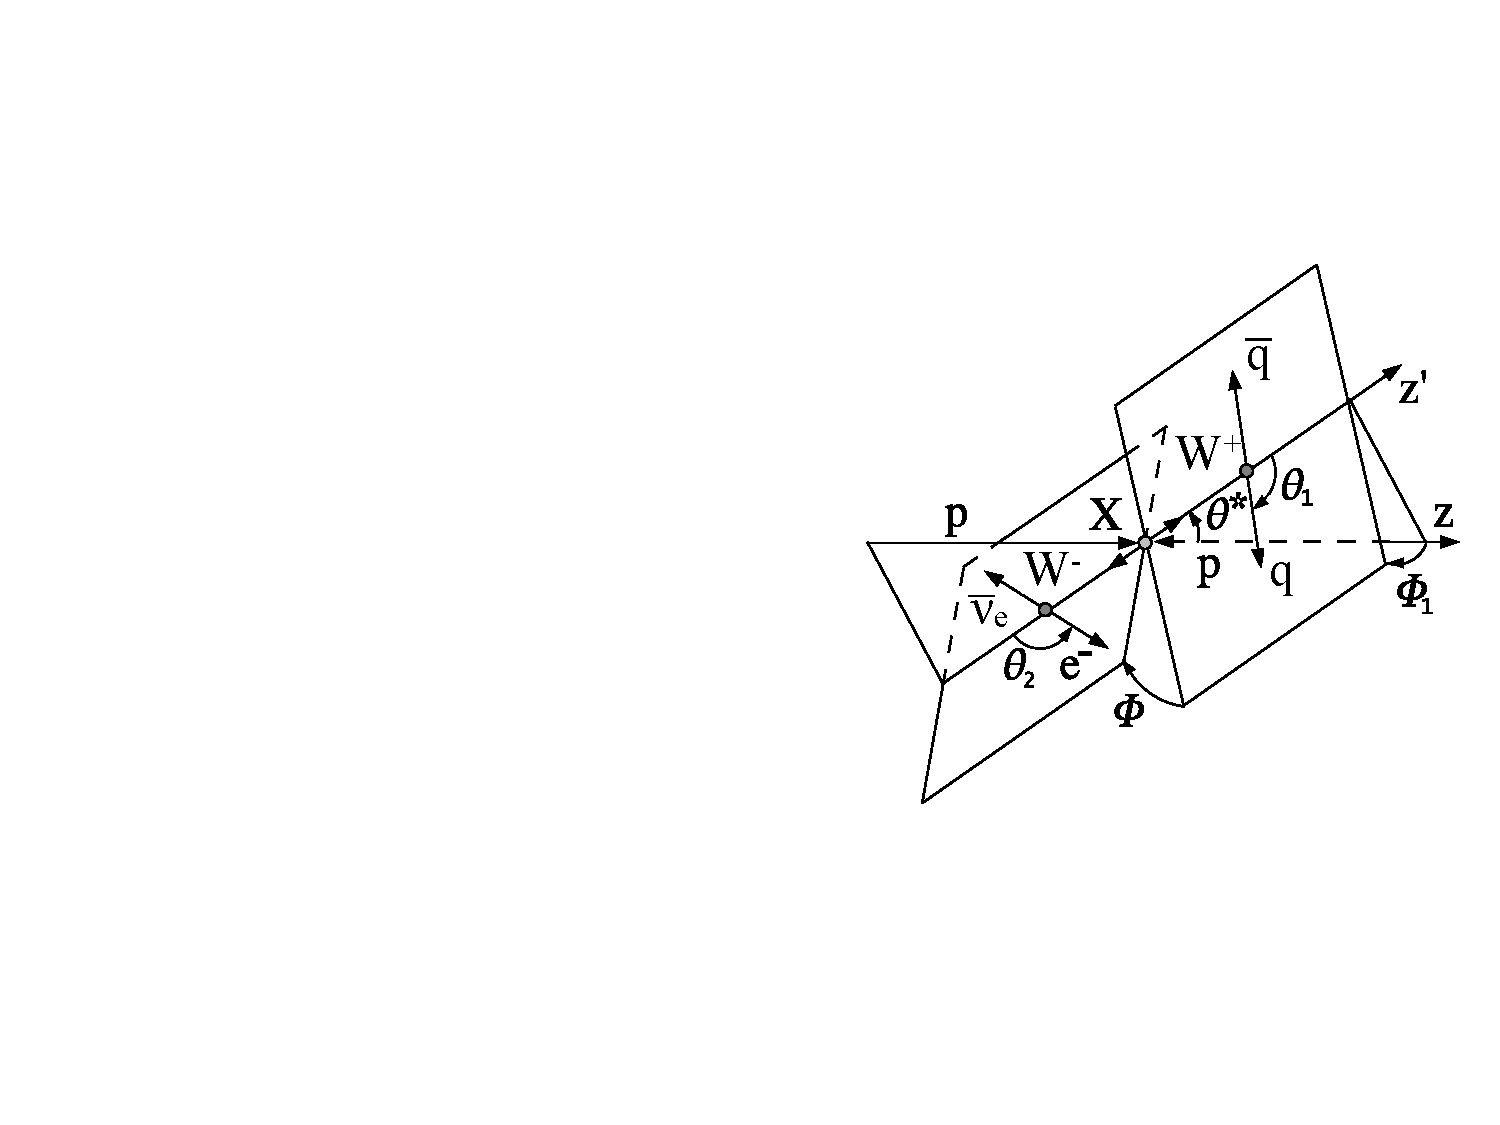
\includegraphics[width=0.5\textwidth]{plots/2012_MVAangles_wwlvjj.pdf}
  \caption{\label{fig:anglesWWlvjj}Angular definition for the $WW\to l\nu jj$ process}
\end{figure}
%%%%%%%%%%%%%%%%%%%
The angle $\cos\theta^{\ast}$ is the polar angle between the parton
collision axis z and the $X$ decay axis $z'$, both defined in the $X$
rest frame. The angle $\Phi_1$ is the azimuthal angle between the
$zz'$ plane and the decay plane of hadronic $W$. The angles
$\cos\theta^{\ast}$ and $\Phi_1$ are denoted as production angles
because they depend on the production mechanism, $gg$ or $q\bar{q}$.
For the SM Higgs which is a spin-zero particle, the production angles
are flat (before acceptance). The angle $\Phi$ is the angle between
the decay planes of the two $W$ systems in the $X$ rest frame. The
angle $\theta_i$ is the angle between the direction of the fermion f
from $W \to f\bar{f}$ and the direction opposite the $X$ in the $W_i$
rest frame, where index i = 1, 2 refers to the first or second $W$
boson.  In the case of the $\cos\theta_i$ angle from the hadronic $W$,
it is ambiguous as to which jet is originating from the fermion or
anti-fermion, so the angles is defined from $0$ to $\pi$ for the
leading $p_T$ jet.  Finally, The angles $\Phi$, $\cos\theta_1$ and
$\cos\theta_2$ do not depend on the production mechanism and are
denoted as the helicity angles.

The observables $m_{l\nu jj}$ and $m_{jj}$ are excluded from the MVA
inputs.  The observable, $m_{l\nu jj}$, is not used because it is the
distribution of this observable which is used in the extraction of the
upper limit.  The observable, $m_{jj}$, is not used since the $m_{jj}$
distribution is used to extract from the sideband to the signal region
to extract a data-driven shape for the background in the $m_{l\nu jj}$
spectrum.  The leaves the five angular variables as inputs to the
multivariate discriminant.  As an example, the related search for the
Higgs in the $ZZ \to 2l2q$ final state at CMS~\cite{CMS2l2q} uses
these five observables in an angular discriminant.  Since the
invariant masses are not used in the multivariate discriminant, the
angular variables are defined in a loose window in $m_{l\nu jj}$ in
order to take into account the correlations between the angles and the
masses.

In addition, to the five angular variables the $p_T$ of the WW system
$p_{T,WW}$ and longitudinal boost (rapidity) $Y_{WW}$ are also used.
The $Y_{WW}$ distribution comes from the parton distribution
functions.  The $p_{T,WW}$ distribution comes from next-to-leading
order effects.  The lepton charge is also included to give some
discrimination power since the $W$ + jets background is asymmetric
with respect to charge while the SM Higgs signal will be symmetric in
lepton charge.  These two quantities in addition to the mass and
angular quantities form a full set of kinematic observables for
process.  Other discriminating observables such as the $p_T$ of the
$W\to jj$ system are not independent of the full set (and particularly
of $m_{l\nu jj}$ and $m_{jj}$) are thus not used since they can sculpt
the invariant mass distributions to make the background more
"signal-like".

%%Finally the quark-gluon likelihood discriminant observables for the two jets are used.  
%%The quark-gluon likelihood discriminant gives a measure of a jet originating from a quark or gluon~\cite{qgAN}
%%The SM Higgs signal consists of quark jets while the background is an admixture of both quark and gluon jets.  
%%
Combining all the inputs together the final set of inputs to the multivariate discriminant is:
\begin{equation}
\{ \cos\theta_1, \cos\theta_2, \Phi, \cos\theta^{\ast}, \Phi_1, p_{T,WW}, Y_{WW}, {\rm lepton~charge}\}
\end{equation}
%As an example, we plot the input variables for the SM Higgs mass of 300~GeV for the $W\to\mu\nu$ category in Fig.~\ref{fig:inputs3002jmu}.


The distributions of input variables are shown in Figs~\ref{fig:inputs170mu}--\ref{fig:inputs600mu}
for all Higgs mass points, muon category.
%%%%%%%%%%%%%%%%%%%
\newpage
\subsection{Input variables: \texorpdfstring{$M_H$}{M(H)} = 170~GeV}
%%%%%%%%%%%%%%%%%%%
\begin{figure}[ht]
  \centering
  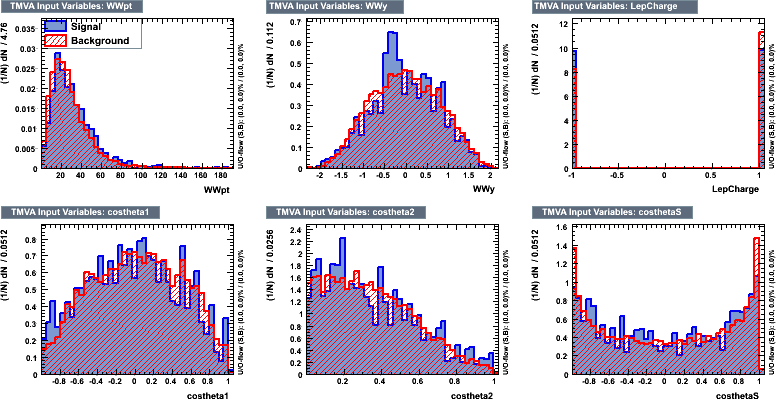
\includegraphics[width=0.9\textwidth]{plots/2012_MVA/TMVA_170_nJ2_mu_variables_id_c1.png}
  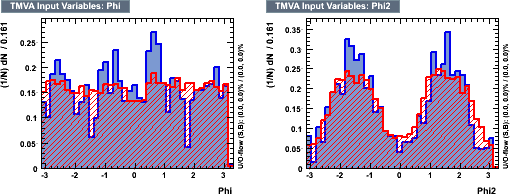
\includegraphics[width=0.6\textwidth]{plots/2012_MVA/TMVA_170_nJ2_mu_variables_id_c2.png}	
  \caption{\label{fig:inputs170mu}Inputs to the multivariate discriminant for $M_H = $170~GeV for the muon category}
\end{figure}
%%%%%%%%%%%%%%%%%%%
\newpage
\subsection{Input variables: \texorpdfstring{$M_H$}{M(H)} = 180~GeV}
%%%%%%%%%%%%%%%%%%%
\begin{figure}[ht]
  \centering
  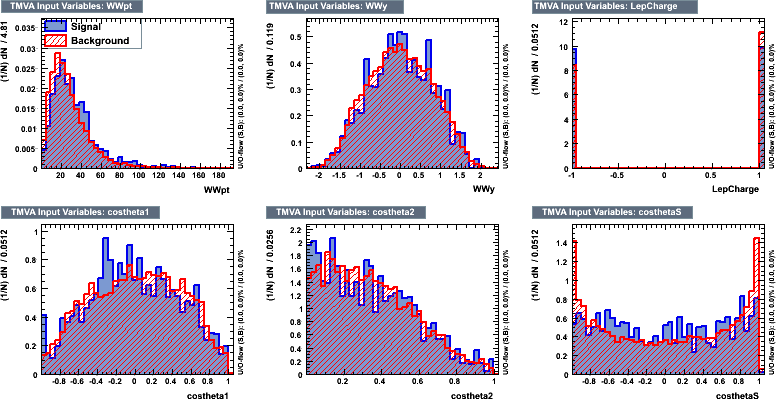
\includegraphics[width=0.9\textwidth]{plots/2012_MVA/TMVA_180_nJ2_mu_variables_id_c1.png}
  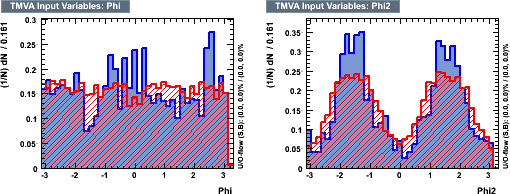
\includegraphics[width=0.6\textwidth]{plots/2012_MVA/TMVA_180_nJ2_mu_variables_id_c2.png}	
  \caption{\label{fig:inputs180mu}Inputs to the multivariate discriminant for $M_H = $180~GeV for the muon category}
\end{figure}
%%%%%%%%%%%%%%%%%%%
\newpage
\subsection{Input variables: \texorpdfstring{$M_H$}{M(H)} = 190~GeV}
%%%%%%%%%%%%%%%%%%%
\begin{figure}[ht]
  \centering
  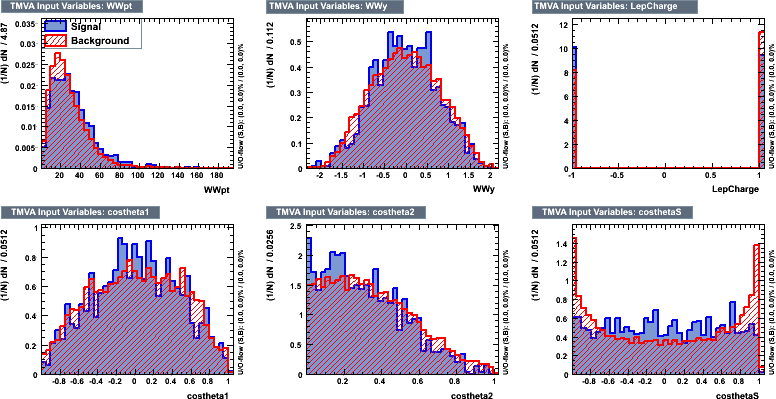
\includegraphics[width=0.9\textwidth]{plots/2012_MVA/TMVA_190_nJ2_mu_variables_id_c1.png}
  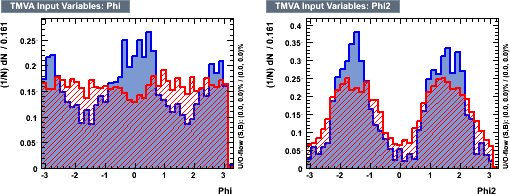
\includegraphics[width=0.6\textwidth]{plots/2012_MVA/TMVA_190_nJ2_mu_variables_id_c2.png}	
  \caption{\label{fig:inputs190mu}Inputs to the multivariate discriminant for $M_H = $190~GeV for the muon category}
\end{figure}
%%%%%%%%%%%%%%%%%%%
\newpage
\subsection{Input variables: \texorpdfstring{$M_H$}{M(H)} = 200~GeV}
%%%%%%%%%%%%%%%%%%%
\begin{figure}[ht]
  \centering
  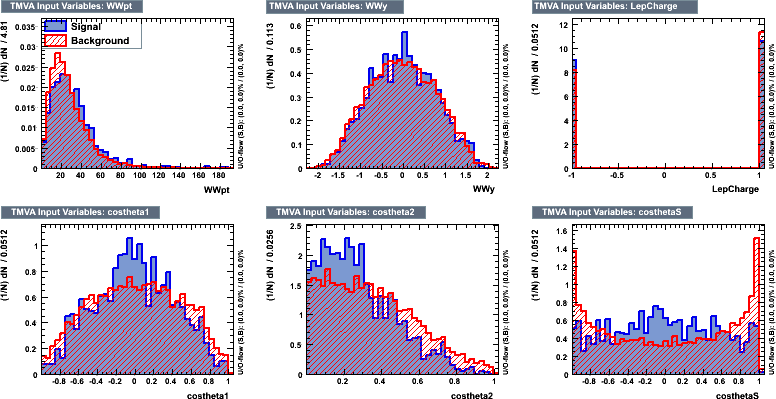
\includegraphics[width=0.9\textwidth]{plots/2012_MVA/TMVA_200_nJ2_mu_variables_id_c1.png}
  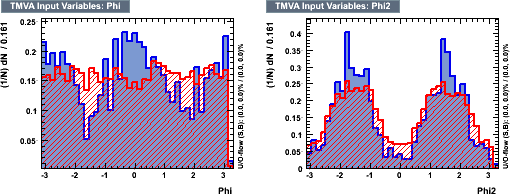
\includegraphics[width=0.6\textwidth]{plots/2012_MVA/TMVA_200_nJ2_mu_variables_id_c2.png}	
  \caption{\label{fig:inputs200mu}Inputs to the multivariate discriminant for $M_H = $200~GeV for the muon category}
\end{figure}
%%%%%%%%%%%%%%%%%%%
\newpage
\subsection{Input variables: \texorpdfstring{$M_H$}{M(H)} = 250~GeV}
%%%%%%%%%%%%%%%%%%%
\begin{figure}[ht]
  \centering
  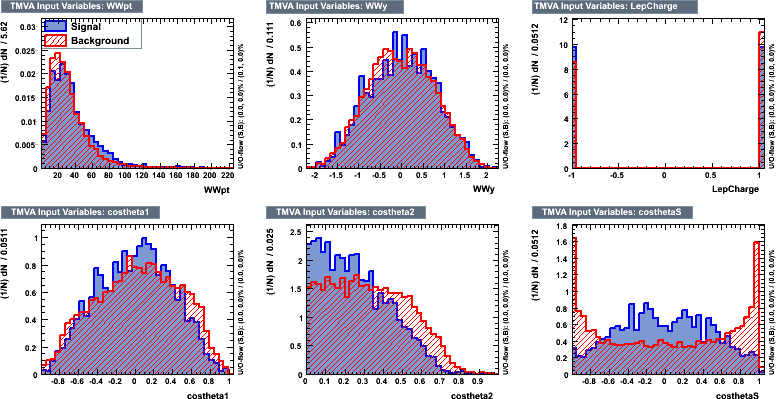
\includegraphics[width=0.9\textwidth]{plots/2012_MVA/TMVA_250_nJ2_mu_variables_id_c1.png}
  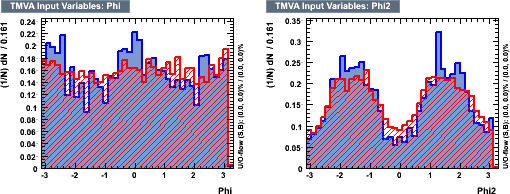
\includegraphics[width=0.6\textwidth]{plots/2012_MVA/TMVA_250_nJ2_mu_variables_id_c2.png}	
  \caption{\label{fig:inputs250mu}Inputs to the multivariate discriminant for $M_H = $250~GeV for the muon category}
\end{figure}
%%%%%%%%%%%%%%%%%%%
\newpage
\subsection{Input variables: \texorpdfstring{$M_H$}{M(H)} = 300~GeV}
%%%%%%%%%%%%%%%%%%%
\begin{figure}[ht]
  \centering
  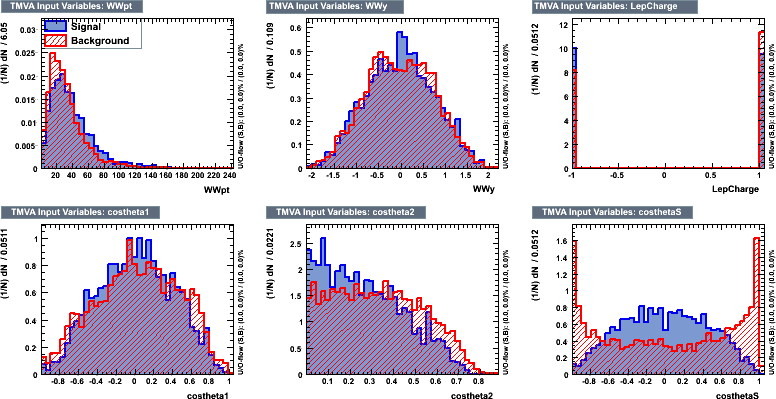
\includegraphics[width=0.9\textwidth]{plots/2012_MVA/TMVA_300_nJ2_mu_variables_id_c1.png}
  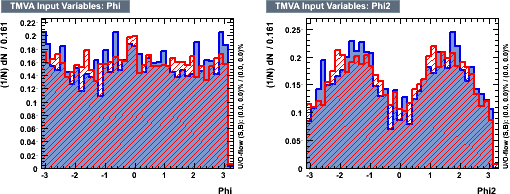
\includegraphics[width=0.6\textwidth]{plots/2012_MVA/TMVA_300_nJ2_mu_variables_id_c2.png}	
  \caption{\label{fig:inputs300mu}Inputs to the multivariate discriminant for $M_H = $300~GeV for the muon category}
\end{figure}
%%%%%%%%%%%%%%%%%%%
\newpage
\subsection{Input variables: \texorpdfstring{$M_H$}{M(H)} = 350~GeV}
%%%%%%%%%%%%%%%%%%%
\begin{figure}[ht]
  \centering
  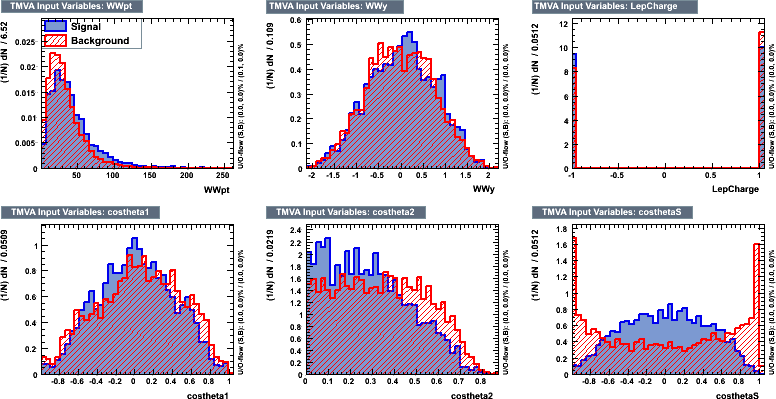
\includegraphics[width=0.9\textwidth]{plots/2012_MVA/TMVA_350_nJ2_mu_variables_id_c1.png}
  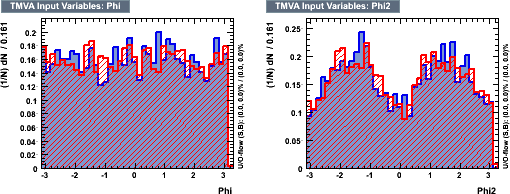
\includegraphics[width=0.6\textwidth]{plots/2012_MVA/TMVA_350_nJ2_mu_variables_id_c2.png}	
  \caption{\label{fig:inputs350mu}Inputs to the multivariate discriminant for $M_H = $350~GeV for the muon category}
\end{figure}
%%%%%%%%%%%%%%%%%%%
\newpage
\subsection{Input variables: \texorpdfstring{$M_H$}{M(H)} = 400~GeV}
%%%%%%%%%%%%%%%%%%%
\begin{figure}[ht]
  \centering
  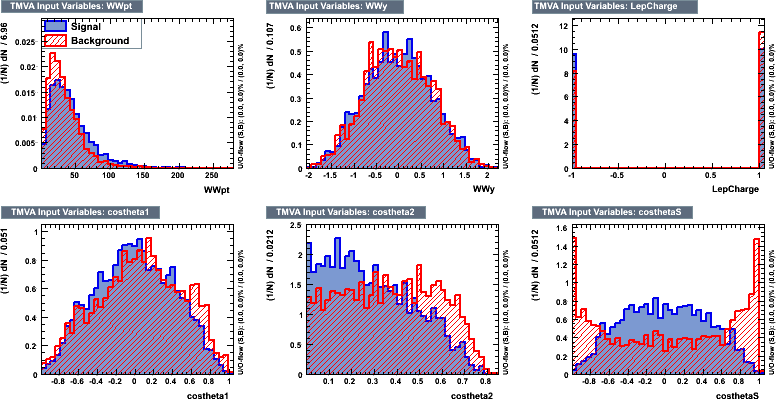
\includegraphics[width=0.9\textwidth]{plots/2012_MVA/TMVA_400_nJ2_mu_variables_id_c1.png}
  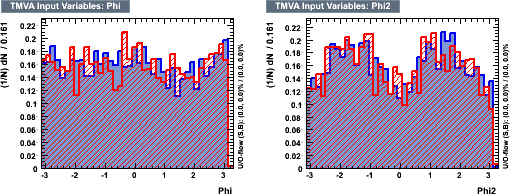
\includegraphics[width=0.6\textwidth]{plots/2012_MVA/TMVA_400_nJ2_mu_variables_id_c2.png}	
  \caption{\label{fig:inputs400mu}Inputs to the multivariate discriminant for $M_H = $400~GeV for the muon category}
\end{figure}
%%%%%%%%%%%%%%%%%%%
\newpage
\subsection{Input variables: \texorpdfstring{$M_H$}{M(H)} = 450~GeV}
%%%%%%%%%%%%%%%%%%%
\begin{figure}[ht]
  \centering
  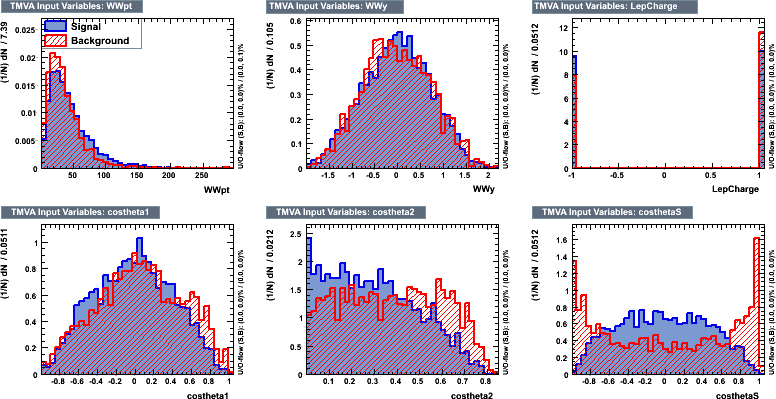
\includegraphics[width=0.9\textwidth]{plots/2012_MVA/TMVA_450_nJ2_mu_variables_id_c1.png}
  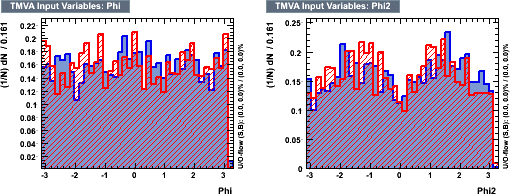
\includegraphics[width=0.6\textwidth]{plots/2012_MVA/TMVA_450_nJ2_mu_variables_id_c2.png}	
  \caption{\label{fig:inputs450mu}Inputs to the multivariate discriminant for $M_H = $450~GeV for the muon category}
\end{figure}
%%%%%%%%%%%%%%%%%%%
\newpage
\subsection{Input variables: \texorpdfstring{$M_H$}{M(H)} = 500~GeV}
%%%%%%%%%%%%%%%%%%%
\begin{figure}[ht]
  \centering
  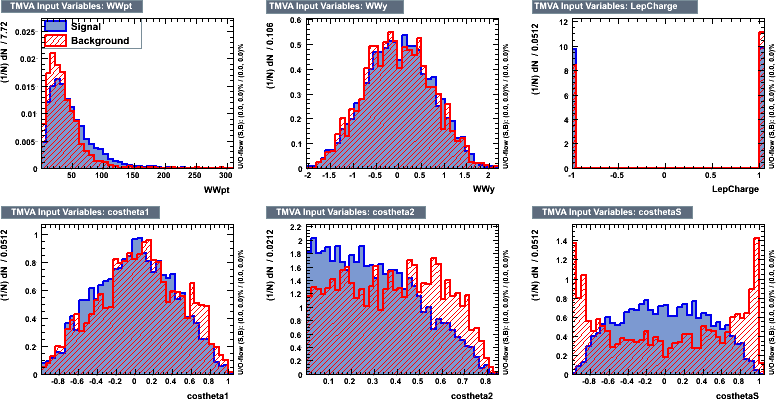
\includegraphics[width=0.9\textwidth]{plots/2012_MVA/TMVA_500_nJ2_mu_variables_id_c1.png}
  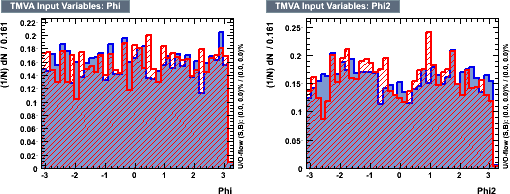
\includegraphics[width=0.6\textwidth]{plots/2012_MVA/TMVA_500_nJ2_mu_variables_id_c2.png}	
  \caption{\label{fig:inputs500mu}Inputs to the multivariate discriminant for $M_H = $500~GeV for the muon category}
\end{figure}
%%%%%%%%%%%%%%%%%%%
\newpage
\subsection{Input variables: \texorpdfstring{$M_H$}{M(H)} = 550~GeV}
%%%%%%%%%%%%%%%%%%%
\begin{figure}[ht]
  \centering
  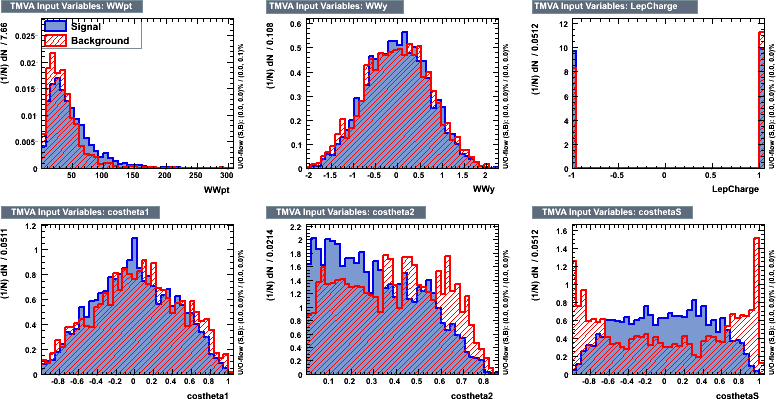
\includegraphics[width=0.9\textwidth]{plots/2012_MVA/TMVA_550_nJ2_mu_variables_id_c1.png}
  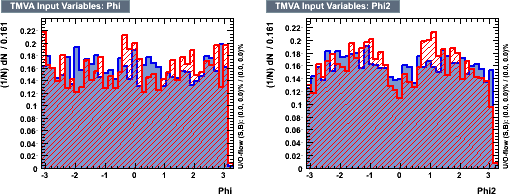
\includegraphics[width=0.6\textwidth]{plots/2012_MVA/TMVA_550_nJ2_mu_variables_id_c2.png}	
  \caption{\label{fig:inputs550mu}Inputs to the multivariate discriminant for $M_H = $550~GeV for the muon category}
\end{figure}
%%%%%%%%%%%%%%%%%%%
\newpage
\subsection{Input variables: \texorpdfstring{$M_H$}{M(H)} = 600~GeV}
%%%%%%%%%%%%%%%%%%%
\begin{figure}[ht]
  \centering
  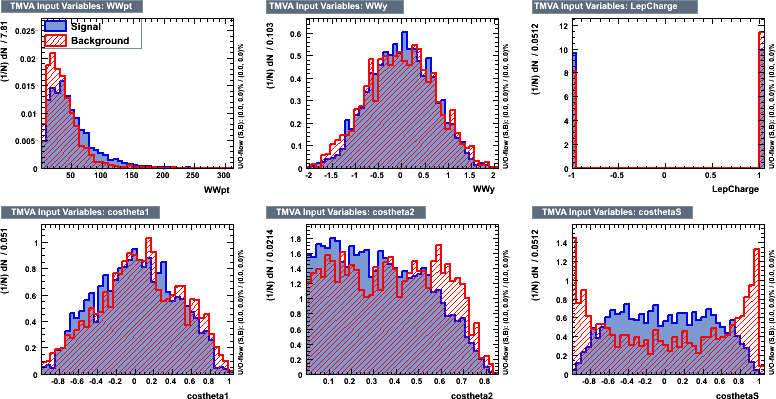
\includegraphics[width=0.9\textwidth]{plots/2012_MVA/TMVA_600_nJ2_mu_variables_id_c1.png}
  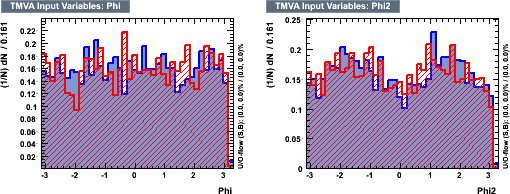
\includegraphics[width=0.6\textwidth]{plots/2012_MVA/TMVA_600_nJ2_mu_variables_id_c2.png}	
  \caption{\label{fig:inputs600mu}Inputs to the multivariate discriminant for $M_H = $600~GeV for the muon category}
\end{figure}
%%%%%%%%%%%%%%%%%%%
%%%%%%%%%%%%%%%%%%%
